
\chapter{DESARROLLO DE APRENDIZAJE}

Capítulo compuesto por todo el trabajo de investigación sobre el trabajo realizado durante los meses de Noviembre hasta Enero inclusive.

Las siguientes secciones se basan en el estudio y comprensión de los artículos relacionados con los autoencoders. En dichas secciones, haré un breve resumen sobre lo entendido.

\section{Autocodificadores para la fusión de características no lineales: Taxonomía, modelos, software y directrices}

Los autoencoders (AEs) nos sirven para la fusión de características de forma no lineal.

Se recogerá una visión amplia de los AEs, su uso para la fusión de características, una taxonomía con diferentes modelos, cómo elegir el autoencoder adecuado para un problema determinado, diferentes softwares, y, por último, unos ejemplos de uso.

\begin{enumerate}
    \item \textbf{Introducción.} 
    \par Los autoencoders (AEs) son Redes Neuronales Artificiales (RNA) que codifican los datos de entrada y son entrenados para que al decodificar dichos datos, sean lo más parecido a las entradas.
    
    Es importante tener en cuenta que, aunque se ha desarrollado para el contexto del aprendizaje profundo, no todos los autoencoders son RNA con múltiples capas ocultas (profundo). Con esto sabemos que el AE puede ser RNA profunda o una RNA superficial con una única capa oculta.
    
    Está claro que debemos de evitar el problema de \textbf{\textit {The Curse of Dimensionality}}, el cual degrada un buen comportamiento de una RNA conforme aumenta el número de variables de entrada. Todo esto, nos lleva al auge en la Ingeniería de características.
    
    La selección del mejor subconjunto de variables de entrada es un problema combinatorio \textbf{NPhard problema combinatorio}. Además, sabemos que la evaluación de forma independiente de las variables nos lleva, dependiendo del problema, a perder información sobre los posibles pesos que existan en las relaciones entre ellas.
    
    A continuación, se obtiene una visión de los diferentes conceptos relacionados con las variables (características) de entrada:
    
    \begin{itemize}
        \item \textbf{Ingeniería de características:} Término global, caracterizado por su uso manual/automatizado de la selección/creación de características de entrada.
        
        \item \textbf{Aprendizaje de características:} Proceso automatizado de selección/creación de variables de entrada. Basado en los algoritmos que se verán posteriormente.
        
        \item \textbf{Aprendizaje de representación:} Basado en el aprendizaje de características, pero centrado en las RNA para automatizar por completo el proceso de \textbf{generación} de características (PLN, imágenes, etc). 
        
        \item \textbf{Selección de características:} Esencial en el preprocesamiento, basada en algoritmos que eligen las variables de entrada más informativas respecto a la/s variable/s de salida (supervisado) o evitando la redundancia entre ellas (no supervisado).
        
        \item \textbf{Extracción de características:} Técnicas como la normalización, la discretización, las transformaciones básicas aplicadas a determinados tipos de datos pertenencen a este término. Existe extracción mediante combinaciones lineales de las originales (PCA, no supervisados, o LDA, supervisados) y no lineales (algoritmos de \hyperlink{https://scikit-learn.org/stable/modules/manifold.html}{aprendizaje de pliegues}).
        
        \item \textbf{Fusión de características:} Pretenden combinar variables para eliminar información redundante e irrelevante a partir de datos multimodales. Varios AEs se enfocarán en dicho aspecto.
        
    \end{itemize}
    
    \newpage
    \item \textbf{Aspectos esenciales de los autoencoders.} \par Los AEs se entrenan para reconstruir su entrada en la capa de salida. 
    
    \begin{itemize}
        \item \textbf{Estructura general.}
            \par A partir de una entrada \textit{x}, se codifica y decodifica dicha entrada para obtener una reconstrucción \textit{r} (ambas deben tener la misma dimensionalidad). Sin embargo, \textit{y} puede tener diferente dimensionalidad.
            
            En la figura ~\ref{AE_3capasE_3capasS}, tenemos un ejemplo de AE con una codificación de 3 capas y otras 3 capas de decodificación (capa central inclusive para ambos procesos).
            
            \begin{center}
                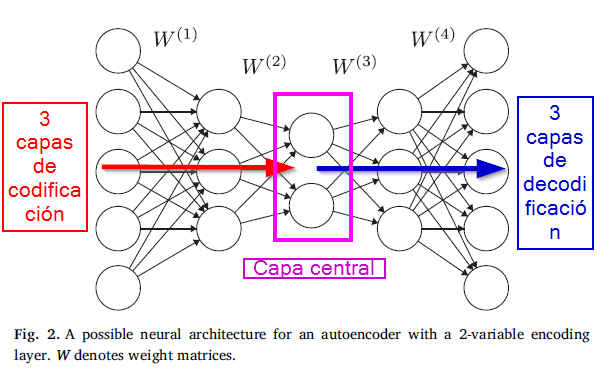
\includegraphics[width=.8\textwidth]{imagenes/AE_3capasE_3capasS.png} 
                \label{AE_3capasE_3capasS}
            \end{center}

        \item \textbf{Funciones de activación de uso común en los autocodificadores.}
            \par Una unidad (nodo) situada en cualquiera de las capas ocultas del RNA obtiene una serie de valores entrantes de la capa anterior y calcula la suma ponderada de estas entradas, obteniendo la elección de la función a usar; es decir, la \textit{\textbf{función de activación}}. A este comportamiento se le considera en las RNA, normalmente, como no lineal.
            Las funciones de activación más comunes y simples son: lineal, binaria, ReLU, logística, tangente y SELU. 
            
            \smallskip
            Las unidades lineales rectificadas (ReLU) son populares en muchos modelos de aprendizaje profundo, pero es una función de activación que tiende a degradar el rendimiento del EA. (Si es negativo, entonces igual 0 y debilita la reconstrucción). Como opción a dicho problema, tenemos la \textit{\textbf{función SELU}}. Por último, tenemos las funciones sigmoides (logística y tangente) que son las más utilizadas.
            
            \begin{center}
                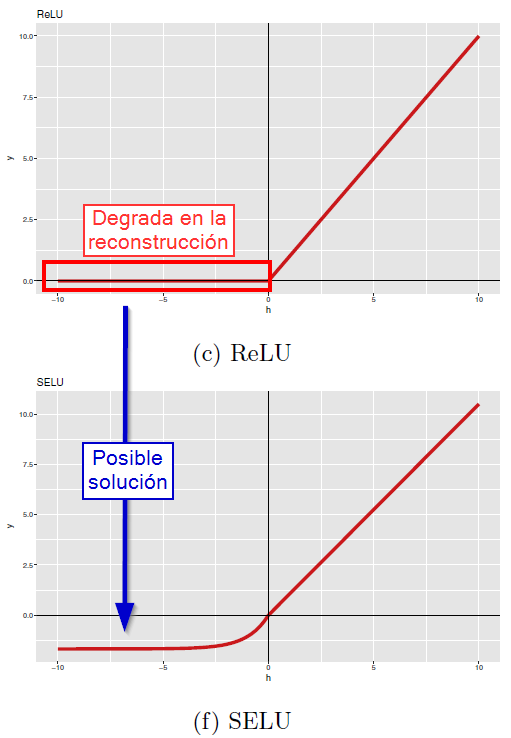
\includegraphics[width=.4\textwidth]{imagenes/Funciones_activacion_ReLU_SELU.png}
            \end{center}
            
        \item \textbf{Grupos de los AEs según la estructura de la red}.
        \par Hay muchas formas de clasificar los AEs, en este momento nos centramos en su estructura.
        
        Los AEs son RNA con una estructura simétrica; es decir, el codificador y decodificador tienen el mismo número de capas con el número de unidades (nodos) por capa con el número inverso [Figura ~\ref{AE_3capasE_3capasS}]. 
        
        Según la \textbf{dimesionalidad} (número de unidades) de la capa de codificación:
            \begin{enumerate}
                \item \textbf{Subcompletos}. Menor número de dimensionalidad (unidades/nodos) que de variables de entrada. Supone una representación compacta obligatoria al AE. Se hace mediante \textit{fusión de características originales} según sus pesos.
                
                \item \textbf{Excesivamente completos}. Dimensionalidad igual o mayor al número de características originales. Existe la posibilidad de replicar la función de identidad, el cual es un problema que debe ser restringido.
            \end{enumerate}
            
        Además, la estructura también depende del \textbf{número de capas}:
            \begin{enumerate}
                \item \textbf{Poco profundo}.Existe sólo una capa oculta (la de codificación).
                
                \item \textbf{Profundo}.Existen más de una capa oculta, el cual puede entrenarse capa a capa o como una RNA profunda.
            \end{enumerate}
        
        \newpage
        La Figura ~\ref{Estructuras_AEs_4tipos} nos muestra las diferentes estructuras explicadas. Rodeado en \color{red}rojo \color{black} está el mismo tipo de estructura según la \color{red}dimensionalidad \color{black} y rodeado en \color{blue}azul \color{black} está según el \color{blue}número de capas \color{black}. Ambos colores, agrupan al mismo tipo correspondiente.
            
        \begin{center} 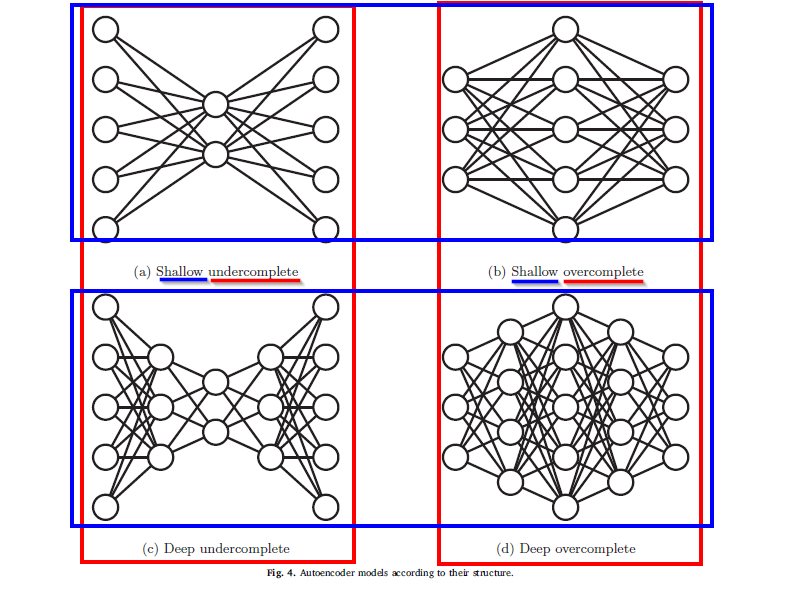
\includegraphics[width=.8\textwidth]{imagenes/Estructuras_AEs_4tipos.png}
        \label{Estructuras_AEs_4tipos}
        \end{center}
        
        \item \textbf{Taxonomía del autocodificador}.
        \par Para explicar la taxonomía, debemos de basarnos en la imagen que viene a continuación. En ella aparecen cuatro pilares:
            \begin{enumerate}
                \item \textbf{Baja dimensionalidad}. No realizan ningún tipo de aprendizaje de características de alto nivel y se ven obligados a optimizar una cantidad notable de parámetros. Esta tarea puede facilitarse simplemente reduciendo la dimensionalidad de los datos, y éste es el objetivo del \textbf{AE básico}.
                
                \item \textbf{Regularización}.A veces, es necesario requerir sobre las características aprendidas unas propiedades matemáticas específicas. 
                
                \item \textbf{Tolerancia al ruido}.Es deseable una alta robustez de los datos frente a datos ruidosos.
                
                \item \textbf{Modelo generativo}.En ocasiones, es útil mapear nuevas muestras en el espacio codificado sobre las características originales.
            
            \begin{center}  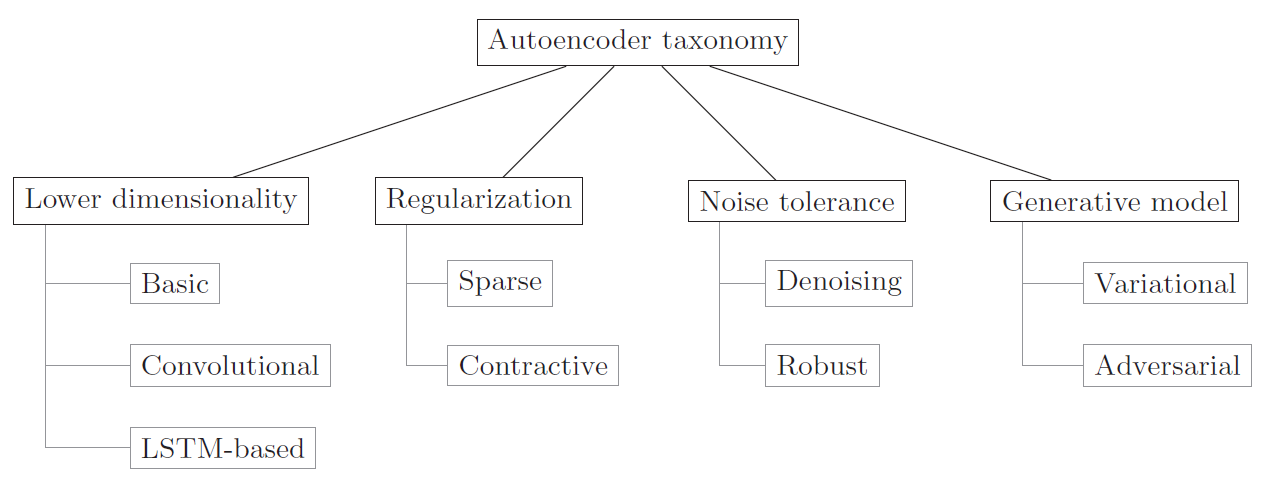
\includegraphics[width=.8\textwidth]{imagenes/AE_Taxonomia.png}
            \label{AE_Taxonomia}
            \end{center}
            
            \end{enumerate}
        
    \end{itemize}
    
    
    \item \textbf{Autocodificadores para la fusión de características.}
    
    \begin{enumerate}
        \item \textbf{Autoencoders básicos}. El objetivo principal de los AEs es el proceso de fusión de características en el que las características aprendidas presentan algunos rasgos deseados (menor dimensionalidad, mayor dispersión, etc). El modelo resultante puede generar nuevas instancias en el espacio de características latentes.
        \begin{enumerate}
            \item \textit{\textbf{Estructura}}. Las capas son de cantidad simétrica en unidades; es decir, las mismas de codificación y decodificación. Pero no necesitan ser simétricas respecto a las funciones de activación o la matriz de pesos.
            
            La más sencilla tiene una única capa oculta, definida por dos matrices de pesos y dos vectores de sesgos:
            \begin{center}
                $y = f(x) = s_{1} (W^{(1)}x + b^{(1)})$,
                
                $r = g (y) = s_{2} (W^{(2)}y + b^{(2)} )$
            \end{center}
            
            Siendo $s_{1}$ y $s_{2}$ las funciones de activación (normalmente, no lineales).
            
            La diferencia respecto a los AEs profundos es que llamaremos a la composición de funciones en el codificador \textit{f}, y la composición de funciones en el decodificador \textit{g}.
            
            \item \textit{\textbf{Función objetivo}}. Se basa en una pérdida por instancia (p.e., error cuadrático medio), por lo que si la función \textit{f} y la función \textit{g} son determinados por la matriz de pesos (\textit{W}) y los sesgos (\textit{b}), necesitamos optimizar \textit{W} y \textit{b} para minimizar la función objetivo.
            
            Por ejemplo, cuando los valores de entrada son
            binarios o modelados como bits, la entropía cruzada suele ser la alternativa preferida
            para la función de pérdida.
            \newpage
        
            \item \textit{\textbf{Entrenamiento}}. Los algoritmos más usados son los basados en la técnica del descenso de gradiente (SGD, o variante de ello). En cada paso, el gradiente de la función objetivo con respecto a los parámetros muestra la dirección de mayor pendiente, y permite al algoritmo modificar los parámetros para buscar un mínimo de la función. Para el cálculo de los gradientes es necesario el \textbf{algoritmo de retropropagación}.
            
            Los AEs son susceptibles al \textbf{sobreajuste}, por lo que se puede aplicar regularización a la función objetivo consiguiendo mayor generalización tras fomentar pesos más pequeños que producen buenas reconstrucciones. De esta forma, los pesos \color{blue}señalados \color{black}  abarcan todos los pesos de W y el $\lambda$ \color{red}señalado \color{black} es un parámetro que determina la magnitud del decaimiento.
            
            \begin{center}
                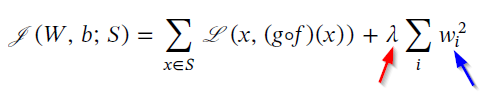
\includegraphics[width=.8\textwidth]{imagenes/AE_basicos_funcion_objetivo_regularizacion.png}
                \label{AE_basicos_funcion_objetivo_regularizacion}
            \end{center}
            
            También existen otras posibilidades como, por ejemplo, provocar simetría entre las matrices de pesos y obtener una reducción de los parámetros consiguiendo eficiencia en los AEs sin alterar la arquitectura deseada.
            
            \item \textit{\textbf{Apilamiento}}. Para los AEs profundos, tenemos la posibilidad de entrenarlos capa por capa; es decir, \textbf{apilar} AEs básicos sucesivamente. Con esto obtenemos una mayor certeza de que los pesos iniciales para los AEs profundos es aceptable (el cuál es muy importante para que el proceso sea existoso).
            
            Aplicamos el entrenamiento capa por capa como se mostrará en la siguiente imagen, donde cada capa es entrenada sucesivamente hasta la codificación.
            \newpage
            
            \begin{center}
                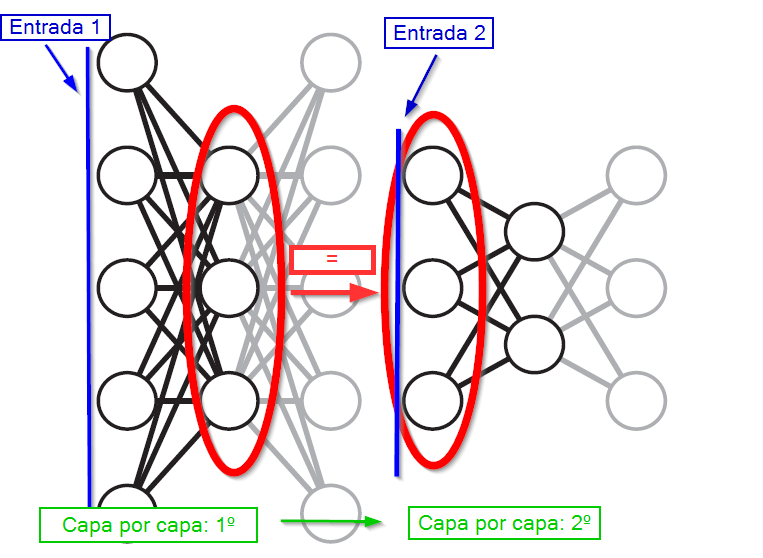
\includegraphics[width=.8\textwidth]{imagenes/AE_apilamiento.png}
                \label{AE_apilamiento}
            \end{center}
            
        \end{enumerate}
        
        \item \textit{\textbf{Regularización}}. En AEs básicos, las codificaciones no presentan propiedades especiales. Cuando queremos que esto ocurra, añadimos a la función objetivo una penalización $\Omega$.
            
            
            \begin{enumerate}
                \item \textit{\textbf{Autoencoders dispersos}}. La escasez en una representación indica que los valores, en su mayoría, dan cero o cercanos a cero. Esto da motivo de uso a las transformacones de muestras en códigos dispersos (sobrecompleto y significativo) en el aprendizaje automático. 
                
                En los AEs básicos, los códigos sobrecompletos serían entrenados para copiar sólamente la entradas en las salidas.
                
                Para añadir la dispersidad en un AE, se añade una penalización a la función de pérdida. Para comparar la activación deseada de una unidad (nodo), estas se pueden modelar con una  \textit{\textbf{variable aleatoria Bernoulli}}, donde sólo puede disparar o no.
                
                \begin{center}
                $\hat{p}_{i} = \frac{1}{|S|} \sum_{x \in S} f_{i}(x)$,
                \end{center}
                
                siendo $\hat{p}_{i}$ la media de la distribución Bernoulli asociada. Con esto, usaremos la \textit{\textbf{divergencia de Kullback-Leibler}}, siendo $p$ la activación media deseada, entre la variable aleatoria definida por la unidad \textit{i} y la correspondiente a las activaciones deseadas medirá la diferencia de distribución.
                
                \begin{center}
                $KL(p||\hat{p}_{i}) = p \log\frac{p}{\hat{p}_{i}} + (1 - p) \log\frac{1 - p}{1 - \hat{p}_{i}}$.
                \end{center}
                \newpage
                
                \begin{center}
                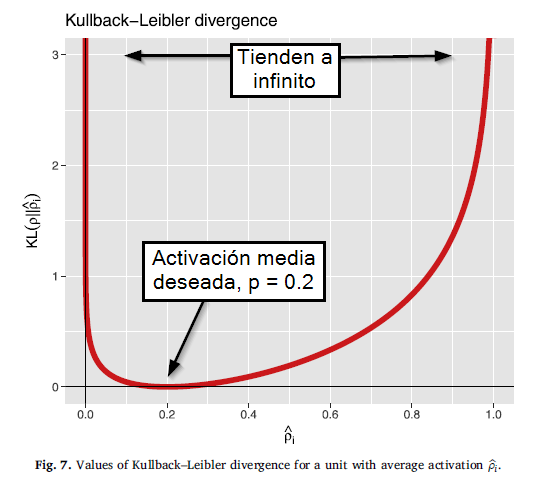
\includegraphics[width=.8\textwidth]{imagenes/AE_Regularizacion_dispersos_BernoulliKullback.png}
                \label{AE_Regularizacion_dispersos_BernoulliKullback}
                \end{center}
                
                Se observa que la penalización es baja cuando la activación media está cerca de la deseada, pero crece rápidamente a medida que se aleja.
                
                Por lo tanto, el término penalizante para la función objetivo es:
                
                \begin{center}
                $\Omega_{SAE}(W,b;S) = \sum_{i = 1}^{c} KL(p||\hat{p}_{i})$,
                \end{center}
                
                donde el valor de la media de activación $\hat{p}_{i}$ depende de lo parámetros del codificador y el conjunto de entrenamiento $S$.
                
                \item \textit{\textbf{Autoencoder contractivo}}. Logra invariabilidad a los cambios en muchas direcciones alrededor de las muestras. Para ello, usamos la \textit{\textbf{norma de Frobenius}} $|| \cdot ||_{F}$ de la matriz Jacobiana del codificador $J_{f}$ (cuanto mayor sea el valor, más inestable) y a partir de esta medida se construye la regularización en la función obtejtivo.
                
                $||J_{f}(x)||_{F}^{2} = \sum_{j = 1}^{d}\sum_{i = 1}^{c} (\frac{\partial f_{i}}{\partial x_{j} (x)})^2$ \hspace{5mm} $\Rightarrow$ \hspace{5mm} $\Omega_{SAE}(W,b;S) = \sum_{x \in S}|| J_{f}(x) ||_{F}^2$
                \newpage
            \end{enumerate}
            
            \item \textit{\textbf{Tolerancia al ruido}}
            \par Un AE puede aprender un espacio de características latente a partir de un conjunto de muestras, pero no garantiza la robustez ante la presencia de instancias ruidosas.
            
            \begin{enumerate}
                \item \textit{\textbf{Eliminación de ruido}}. Un DAE (Denoising AE) aprende a generar características robustas a partir de las entradas reconstruyendo las muestras parcialmente destruidas.
                
                Se aplica una técnica de corrupción estocástica en la fase de entrenamiento, basada en elegir aleatoriamente una cantidad fija de características para cada muestra de entrenamiento y ponerlas a 0 (u otros como el ruido gaussiano, el ruido de \textit{salt-and-pepper}). Los AEs se comparan con las originales y se entrenan para adivinar los valores perdidos.
                
                Un DAE no necesita más restricciones o regularizaciones para aprender una codificación significativa (es decir, puede ser sobrecompleto si se quiere).
                
                Además, se puede aplicar capa por capa para los AEs profundos. Para ello, las entradas no corrompidas se calculan como salidas de las capas anteriores. Entonces, estas entradas se corrompen y se proporcionan a la red.
                
                \begin{center}
                    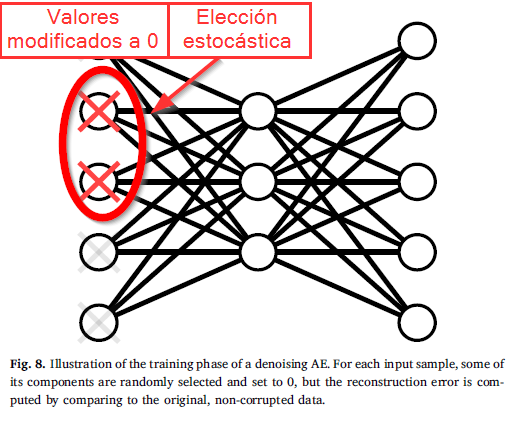
\includegraphics[width = .4\textwidth]{imagenes/AE_ToleranciaRuido_EliminacionRuido.png}
                \end{center}
                
                \item \textit{\textbf{Autoencoder robusto}}. Basado en modificar la función de pérdida utilizada para minimizar el error de reconstrucción y neutralizar la sensibilidad a los distintos tipos de ruido.
                
                Se desarrolla a partir de una función de pérdida diferente, basada en la correntropía; es decir, medir específicamente la densidad de probabilidad de que dos eventos sean iguales. Se trata de minimizar dicho entropía negativa (maximizar) para obtener una mayor resistencia al ruido (sobretodo, el gaussiano).
                
            \end{enumerate}
            \newpage
            
            \item \textit{\textbf{Autoencoders específicos de dominio}}.
            \par Los siguientes AEs son de tipo estándar, pero específicos para modelar imágenes y secuencias.
            
            \begin{itemize}
                \item Autoencoder convolucional. AE estandar no considera la estructura bidimensional al procesar datos de imágenes. Por eso, los convolucionales lo resuelven usando capas totalmente conectadas. 
                
                \item Autoencoder LSTM. AE estandar no está preparado para modelar datos secuenciales, un AE LSTM lo consigue colocando unidades de memoria de largo plazo (LSTM) como codificador y decodificador de la red. El codificador
                LSTM lee y comprime una secuencia en una representación de tamaño fijo
                a partir de la cual el decodificador intenta extraer la secuencia original en
                orden inverso.
            \end{itemize}
            
        \item \textit{\textbf{Modelos generativos}}.
        \par Aprenden una distribución para poder extraer nuevas muestras (instancias), diferentes de las observadas. 
        
        \begin{itemize}
            \item Autoencoder variacional. Sustituyen las funciones deterministas en el codificador por mapeos estocásticos, calculando la función objetivo en virtud de las funciones de densidad de las variables aleatorias. 
            
            \begin{center}
                $\mathcal{L}_{VAE}(\theta,\phi;x) = KL(q_{\phi}(y|x)||p_{\theta}(y)) - \mathcal{E}_{q_{\phi}(y|x)}[\log p_{\theta}(x|y)]$,
            \end{center}
            donde $q$ es la distribución que aproxima la verdadera distribución latente de y, y $\theta$, $\phi$ son los parámetros de cada distribución.
            
            \item Autoencoder adversial. Modela la codificación imponiendo una distribución a priori, entrenando después un AE estándar y simultáneamente, una red discriminativa que intenta distinguir codificaciones a partir de muestras de la previa impuesta. Dado que el codificador se entrena para engañar al discriminador, las codificaciones tenderán a seguir la distribución impuesta.
        \end{itemize}
        
        \item \textit{\textbf{Otros AEs más allá de la fusión de características}}.
        \par Los siguientes AEs no entran en ninguna categoría anterior.
        
        \begin{itemize}
            \item Autoencoder relacional. Los AEs básicos no consideran explícitamente las relaciones entre instancias. Estos AEs relacionales modifican la función objetivo para tener en cuenta la fidelidad de la reconstrucción de las relaciones entre las muestras.
            \newpage
            
            \item Autoenconder discriminativo. Discrimina reuniendo las muestras positivas; es decir, realiza una mejor reconstrucción de la s instancias positivas que de las negativas. Para ello, se optimiza la función de pérdida (\textit{Hinge loss function}). Su objetivo se basa en la detección del objeto.
            
        \end{itemize} 
        
        \item \textit{\textbf{Arquitecturas basada en AEs para el aprendizaje de características}}.
        \par Los AEs básicos sirven como base para crear otras arquitecturas más complejas dedicadas a la \textbf{fusión de características}.
        
        \begin{itemize}
            \item Los árboles autoenconders. El codificador y decodificador son árboles de decisión, con \textbf{nodos de decisión suaves} (progagan sus instancias a todos los hijos con diferentes probabilidades).
            
            \item Autoencoder dual. Intenta aprender 2 representaciones latentes cuando en el problema las variables pueden ser tratadas como instancias y viceversa.
            
            \item Autoenconder relacional o correlación cruzada. Incorpora capas en las que las unidades se combinan por \textbf{multiplicación} en lugar de suma ponderada, ya que representa las correlaciones entre los componentes de sus entradas.
            
            \item Autoencoder recursivo. Árbol construido a partir de los AEs, donde se añade piezas de entrada (reconstruye) a medida que el modelo profundiza. Arquitectura usada para modelar el sentimiento en las frases.
        \end{itemize}

    \end{enumerate}
    
    
    
\end{enumerate}


